\begin{figure*}[h]
  \centering
  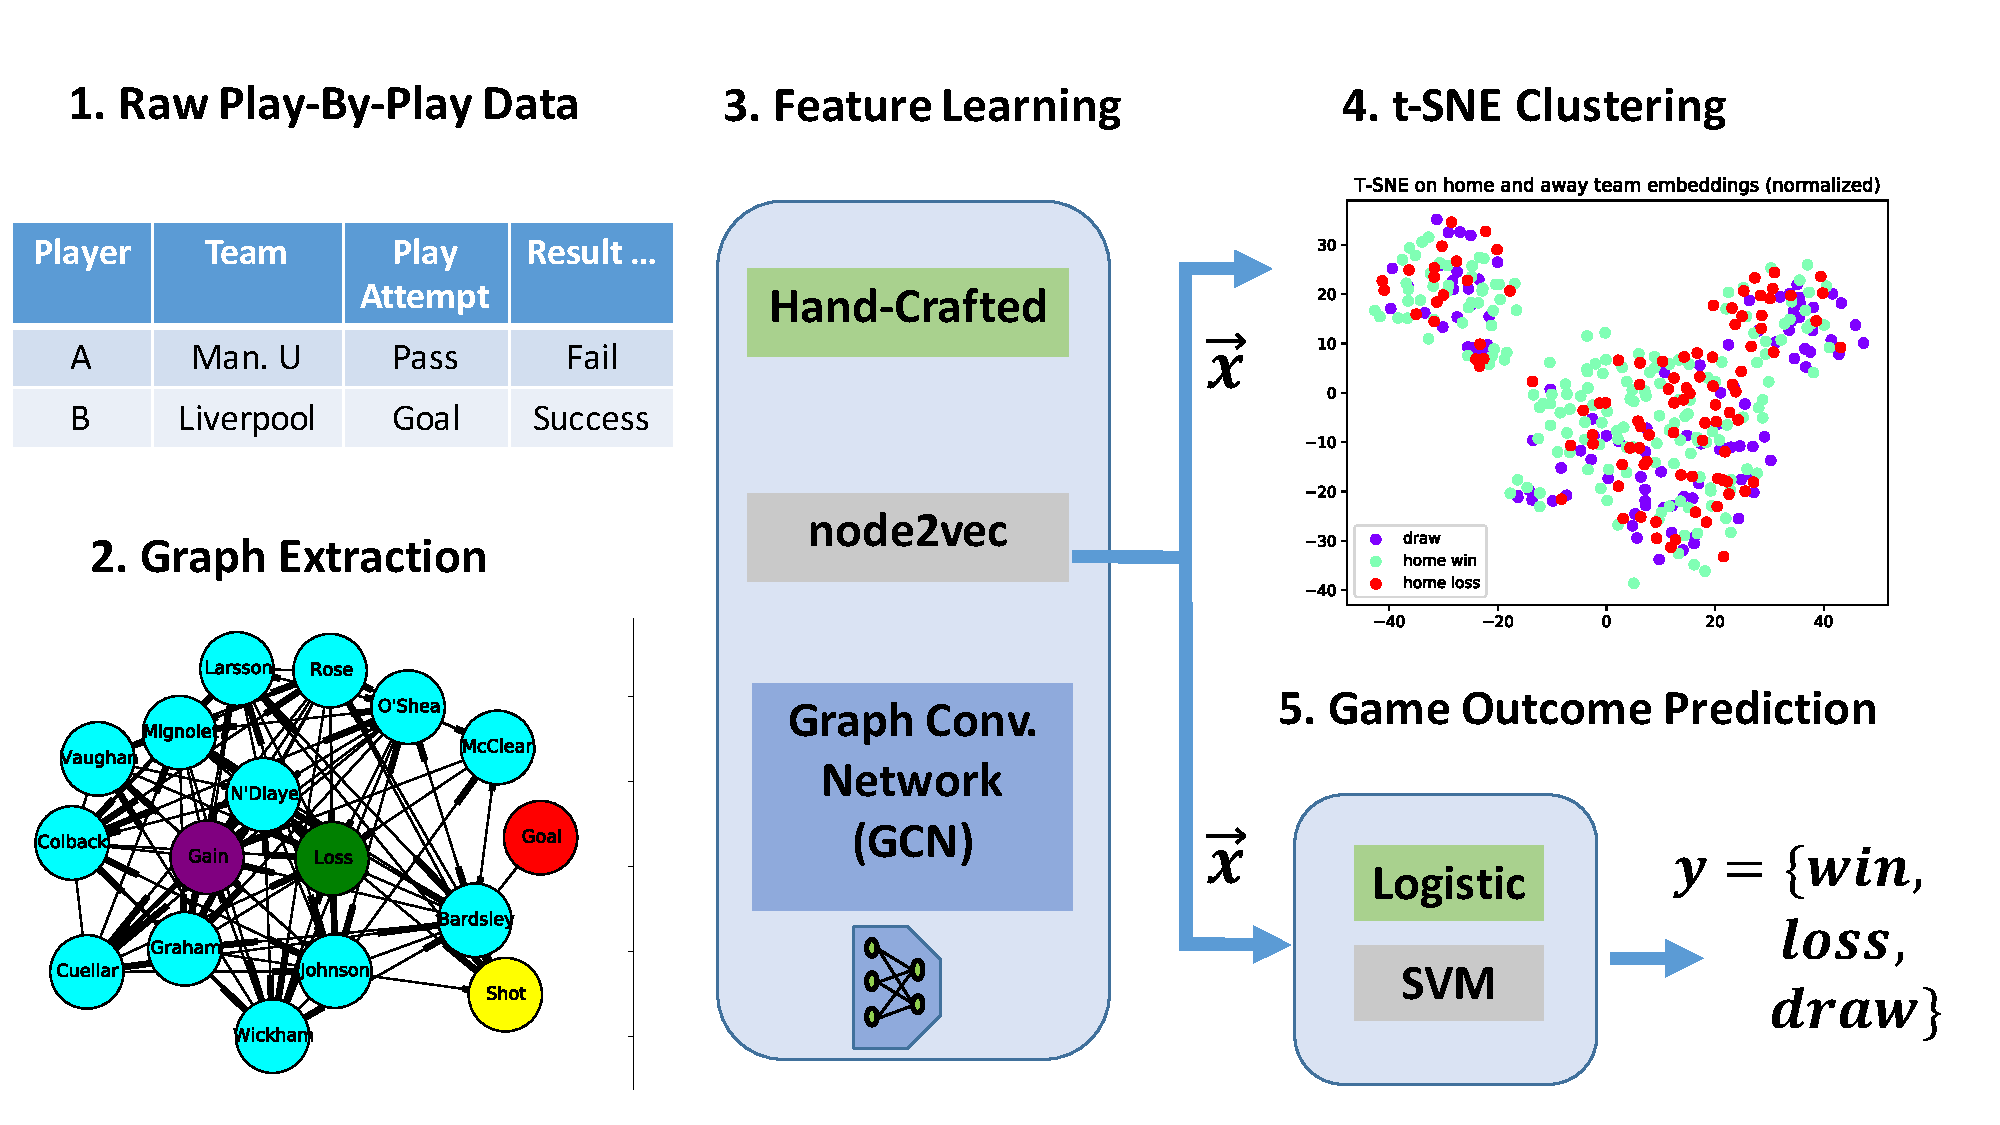
\includegraphics[width=0.95\textwidth]{plots/soccer_block_diagram.pdf}
  \caption{Soccer network analysis pipeline starting from (1) play-by-play data, (2) passing rate graph extraction, (3) feature embedding, (4) clustering, and finally (5) game result prediction. We compared the predictive utility of simple, domain-specific features with complex ones learned by Graph Convolutional Networks (GCNs).}
\end{figure*}

\subsection{Feature Learning: Node Embeddings}
Given our goal to predict game results and/or analyze teams effectively, we want to learn node embeddings from our graphs. So far, we've performed two types of node embeddings with one of them as a baseline. Our goal is to keep working with different embedding strategies and parameters to increase both predictive and classifying powers. 

Our first embedding, which we call simple or hand-crafted features, sets the average pass rate, max pass rate, min pass rate (nonzero), shot rate, gain rate, and loss rate in a vector for each node. We then can assemble a feature vector for a specific graph by averaging the features of the node within the graph. 

Our second embedding uses node2vec with default parameters (128 dimensions, 80 length walk, 10 walks per source, weighted directed graph) to retrieve a feature vector per node. The feature vectors are then averaged to obtain a feature vector for a graph. 

Our current node aggregation technique is simple, but may lose a lot of information. 
Therefore, we hope to learn more rich, higher-order interactions between players, using a more complex model such as a  GCN.

\subsection{Graph Clustering Based on Feature Vectors}
Given both simple hand-crafted features and those from node2vec per team, we wish to cluster them to discover latent relationships or whether they aggregate based on outcome (`win', `loss', `draw') or team identity. Since each team plays 20 games, we have several realizations of a team's playing style.

We used the standard t-SNE method for clustering since it can be projected to two dimensions for easy visualization. Further, its probabilistic assignment of cluster membership is attractive in the soccer context since teams likely have dynamic playing styles based on their opponent, current substitutions, and even whether they are the home team.

We implemented t-SNE using python's  sklearn package and visualized the embeddings in two dimensions for both simple and node2vec features. Per feature set, we ran t-SNE twice, once on a matrix where rows where matches and columns where a single team's features, and again where rows where matches and columns concatenated both the home and away team's vectors. The latter is more useful to predict outcome since it contrasts the playing style of both teams.

We rigorously applied t-SNE using best practices such as sample normalization to account for the different scales of input variables. Initially, we found a few clusters, though they did not separate based on our desired goal of predicting game outcome.


Upon further analysis of nodes in each cluster, we realized that the clusters corresponded to cases where teams had 14,15,16, or 17 players overall due to substitutions. Also, we sometimes saw two clusters, which were later learned to be for `home' and `away' games but were still not predictive of game result. Examples of such uninformative clusters are provided below. 

\begin{figure}[h]
  \centering
  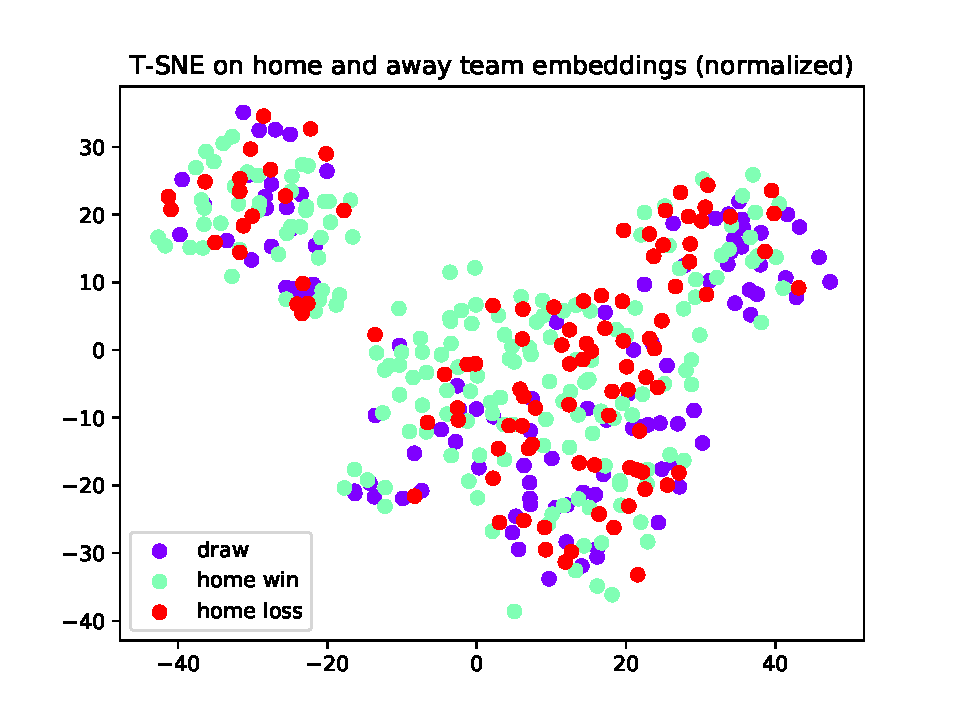
\includegraphics[width=0.45\textwidth]{plots/game_NORM_tsne.pdf}
  \caption{T-SNE shows uninformative clusters based on number of players and home/away status.}
\end{figure}


However, when omitting number of players or home/away team status, we realized t-SNE did not help in clustering the data, as shown below. 
Crucially, rather than simply averaging individual player feature vectors, we 
will subsequently learn more predictive features from them using GCNs.


\begin{figure}[h]
  \centering
  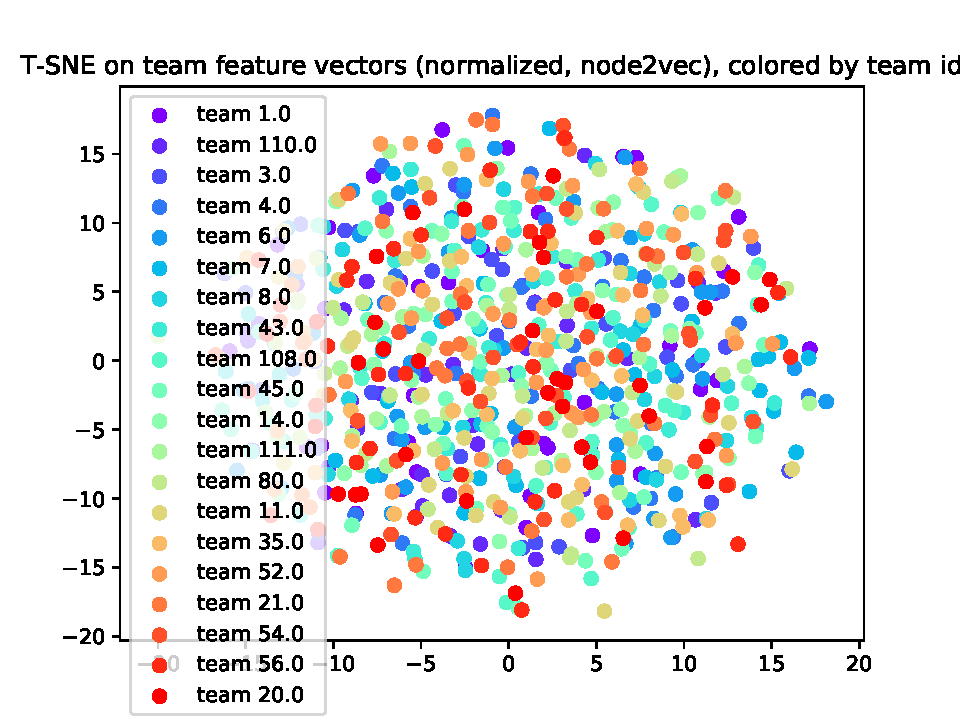
\includegraphics[width=0.45\textwidth]{plots/node2vec_NORM_game_team_teamId_tsne.pdf}
  \caption{T-SNE without confounding features illustrates game result and team styles are hard to predict with current feature vectors.}
\end{figure}


\subsection{Game Result Prediction using Feature Vectors}
Despite the t-SNE results showing minimal predictive power for the current feature vectors, we implemented a simple logistic regression (LR) model that modelled multinomial game outcome based on a concatenation of home team and away team's feature vectors. We employed stratified sampling based on team ID to ensure each team had fair representation both in the training dataset of 304 matches and testing set of 76 matches. 

For simple feature vectors, the LR test set accuracy was 43\% and 48\% on training data. For node2vec features, the performance was similarly bad, with test set accuracy of 38\%. 

As a sanity check of our LR implementation, including the goal differential to predict game outcome yielded 100\% accuracy, but obviously this variable cannot be used. Overall, our results indicate we needed richer features, need to learn higher order interactions between players, and incorporate data from many other leagues besides the EPL.

%\subsection{Addressing Comments from Project Proposal}
%The principal comment from the project proposal, where we wanted to use Graph CNN approaches, was to try node2vec and non deep-learning based approaches due to our limited dataset size. Further, the reviewers anticipated predicting game results to be hard and to focus on clustering teams via learned node features. 
%
%As suggested, we used intuition on soccer dynamics and node2vec to create features and cluster them, which still were not predictive of game results. However, we plan to use significantly more data from several leagues, which allows us to cluster diverse playing styles. Further, we will analyze the temporal nature of each game by creating different passing rates per time window. We find this idea promising since it elicits various playing styles, such as being conservative at the start of a game to aggressive when a team is losing and there is minimal time left.
%
%
%
%
